\subsection{Somatosensorik des Kopfes (trigeminales System) \index{System! trigeminal}}
\label{sec:somatokopf}
Die Somatosensorik des Kopfes beinhaltet beim Menschen die Informationen aus den somatosensorischen Rezeptoren von Gesicht und Mund. Bei einigen Säugetieren kommen noch wichtige Informationen aus den Vibrissen im Gesichtsbereich hinzu. Die Verarbeitung dieser Informationen über das trigeminale System wird im Folgenden beschrieben. Auf die Rolle der Vibrissen wird genauer eingegangen.

\subsubsection*{Vibrissen}
Die Aufgabe von Vibrissen\index{Vibrissa} ist die Nahorientierung und -erkundung, weshalb sie an verhaltensrelevanten Körperteilen vorkommen. Die meisten Säuger, die ihre Nahrung mit der Schnauze ergreifen und nicht mit den Händen, besitzen Vibrissen im Kopfbereich um die Schnauze. Aber auch an anderen Körperstellen, wie z.B. unter dem Kinn (Wüstenspring-mäuse) oder zwischen den Zehen (Katzen), gibt es diese Tasthaare. Die Vibrissen sind lange, steife Tasthaare, welche von einem Blutsinus umgeben sind. Die Schnurrbarthaare \index{Schnurrbarthaare|see{Vibrissa}} sind spezialisierte Vibrissen, die zusätzlich noch bewegt werden können. 
Die Auslenkung der Vibrissen führt zu einer Aktivierung der freien Nervenendigungen, die im Haarschaft zwischen Haar und Blutsinus liegen \textsuperscript{\cite[Kap.~5]{heldmaier2003tierphysiologie}}.

\subsubsection*{Nucleus des Trigeminus}

Die freien Nervenendigungen der Vibrissen und des Mechanorezeptors im Gesicht und Mund bilden gemeinsam einen Teil den fünften Hirnnerv (\textit{Nervus trigeminus})\index{Hirnnerven! 05. N. trigeminus}. Die Ganglien der Nerven liegen alle außerhalb des Hirnstamm im \textit{Ganglion Gasseri} (eng.: trigeminal ganglion)\index{Ganglion Gasseri}, wobei eine Großzahl der Neurone die Vibrissen repräsentiert.
\\
\noindent
Der Trigeminus ist der fünfte Hirnnerv (CN~V). Je nach Lage in den Schnitten durch das Gehirn ist die Bezeichnung des Trigeminus unterschiedlich. Auf der Höhe der Medulla ist es noch der spinale Trakt des Trigeminus (sp5, Abb.~\ref{fig:somato_Pr5}), wohin gegen auf der Höhe des Aquädukts im Mesencephalon von dem sensorischen Trigeminus \index{Trigeminus} (s5, Abb.~\ref{fig:somato_Pr5}) die Rede ist. Der Trigeminus ist auch in sich geordnet, wobei die Neurone aus dem Tastsinn vorne im Trigeminus repräsentiert sind und die Neurone aus dem Schmerzsinn hinten.
\\
\noindent
Die Axone des Ganglion Gasseri ziehen auf der Höhe des Pons in den Hirnstamm und teilen sich dort, um in den Nucleus principalis des Trigeminus (Pr5, \textit{Nucleus principalis nervi trigemini}) \index{Nucleus! principalis, Pr5} und die drei Gebiete des spinalen Nucleus des Trigeminus (Sp5, \textit{Nucleus spinalis nervi trigemini}) \index{Nucleus! spinalis, Sp5}, oralis (Sp5O), interpolaris (Sp5I) und caudalis (Sp5C) zu ziehen. Alle Gebiete gehören zum \textit{Nucleus trigemini}, welcher sich über das Mesencephalon, den Pons und die Medulla erstreckt \textsuperscript{\cite[Kap.~5]{heldmaier2003tierphysiologie}}. 
Hinzu kommen Informationen aus dem Nervus facialis (CN~VII),\index{Hirnnerven! 07. N. facialis} dem Nervus glossopharyngeus \index{Hirnnerven! 09. N. glossopharyngeus} (CN~IX) und dem Nervus vagus (CN~X), welche die Hautbereiche um die Ohren, sowie die Nasen und Rachenregion abdecken
\textsuperscript{\cite[Kap.~12]{neurowissenschaften_baer}}.
\\
\noindent Die Neurone des Nucleus principalis reagieren auf Reize aus dem Kopfbereich, der Zunge und des Gesichts. Zusammen mit dem Nucleus gracilis und Nucleus cuneatus repräsentieren die drei Nuclei den somatosensorischen Input des gesamten Körpers. Die Neurone im Nucleus principalis (Pr5, Abb.~\ref{fig:somato_Pr5}), und in Teilen auch die des Nucleus spinalis (Sp5, Abb.~\ref{fig:somato_Pr5}), bekommen die Information aus spezifischen Körperregionen und sind durch Neuropil in Cluster geteilt. Die Cluster, die aus den einzelnen Vibrissa gebildet werden sind, in der richtigen Schnittebene, gut zu sehen. Sie werden nach dem Zusammenhang mit den 'Barrels' im Cortex, im Nucleus principalis 'barrelettes' genannt \textsuperscript{\cite[Kap.~5]{heldmaier2003tierphysiologie}}.

\begin{figure}[H]
    \centering
    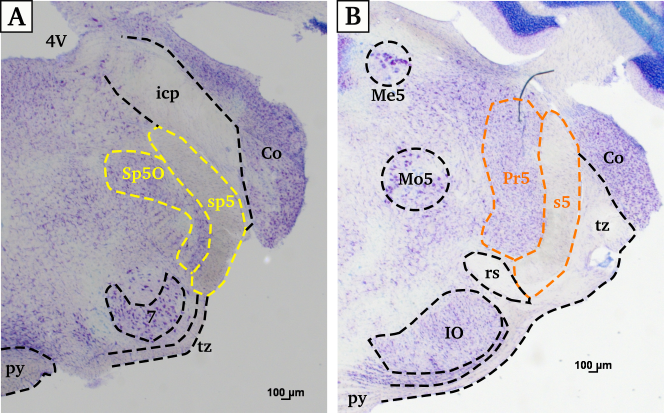
\includegraphics[width = \textwidth]
    {pictures/somatosensory/somato_kopf.png}
    \caption[Nucleus spinalis und Nucleus principalis des Trigeminus]{\textbf{Nucleus spinalis und Nucleus principalis des Trigeminus.}\\
     \textbf{A:}~(N06-4): Der Nucleus spinalis oralis (Sp5O) liegt in der Medulla, lateral auf der Höhe des Nucleus cochlearis (Co) und doral des Nucleus facialis (7). Des weiteren sieht man den spinalen Trigeminus (sp5) lateral dieses Nucleus. Weitere Strukturen sind der vierte Ventrikel (4V), das inferiore cerebellare Pedunkel (icp), die Pyramidenbahn (py) und der Trapezkörper (tz).
     \textbf{B:} (N09-3): Der Nucleus principalis (Pr5) des Trigeminus liegt im Mesencephalon lateral-dorsal auf Höhe der inferioren Olive (IO). Die Axone zum diesem Nucleus liegen im Trigeminus (s5). Weitere Strukturen sind der Nucleus cochlearis (Co), der Nucleus mesencephalicus des Trigeminus (Me5), der Nucleus motorius des Trigeminus (Mo5),  die Pyramidenbahn (py), der rubrospinale Trakt (rs) und der Trapezkörper (tz).}
    \label{fig:somato_Pr5}
\end{figure}

\subsubsection*{Nucleus mesencephalicus des Trigeminus}
Einige der Neurone, die für die somatosensorische Reizweiterleitung aus dem Kopfbereich zuständig sind, haben ihre Zellkörper nicht im Ganglion Gasseri. Dazu gehören die Neurone, die aus den Muskelspindeln kommen, sowie einige Neurone aus den Vibrissen und die Neurone der Zahnwurzeln. Die Zellkörper diese Neurone sind im Nucleus mesencephalicus des Trigeminus (Me5, Abb.~\ref{fig:somato_Pr5}) \index{Nucleus! mesencephalicus, Me5}lokalisiert. Die Axone dieser Neurone projizieren in den dorsomedialen Bereich des Nucleus principalis \index{Nucleus! principalis, Pr5} \textsuperscript{\cite[Kap.~5]{heldmaier2003tierphysiologie}}.

\subsubsection*{Thalamus und Cortex}
Die Axone aus dem Nucleus principalis kreuzen die Mittellinie, stoßen zum medialen Lemniscus hinzu und ziehen in den Thalamus. Die Axone aus dem trigeminalen System ziehen in den medialen Part des Thalamus. Im Thalamus wird über synaptische Verschaltung die Information an die Nervenzellen der thalamocortikalen Verbindung zum primären somatosensorischen Cortex (S1) \index{Cortex! primär somatosensorisch}weiter gegeben. 
Wie schon in Kapitel \ref{subsubsec:S1} beschrieben, ist S1 für die Verarbeitung der somatosensorischen Reize aus dem Körper verantwortlich. Bei Ratten kommen die meisten somatosensorischen Informationen aus den Vibrissen. Von jeder Vibrisse gehen etwa 100 myelinisierte Nervenfasern ab. Über den Trigeminus werden die Informationen zuerst in den Nucleus principalis geleiten. Von dort aus ziehen andere Neurone weiter in den Thalamus und von dort in den Cortex. Die Neurone enden im Cortex \index{Barrel-Cortex} \index{Cortex! Barrel-Cortex} in abgegrenzten Strukturen, den sogenannten 'Barrel' (Abb.~\ref{fig:barrelcortex}~B). Die Anzahl der 'Barrels' entsprechen den der Vibrissen und die 'Barrels' sind nach ihrem Aufbau benannt ('barrels', engl. für Tonnen ): In der Nissl-Färbung (Abbildung~\ref{fig:barrelcortex}~C) sieht man die Neurone dicht gepackt um weniger dichte Bereiche. Die Wände der Tonnen bestehen aus dicht gepackten Neuronen, das Innere aus weniger dicht gepackten Bereichen \textsuperscript{\cite[Kap.~8]{smith2008biology}}. 

\begin{figure}[H]
    \centering
    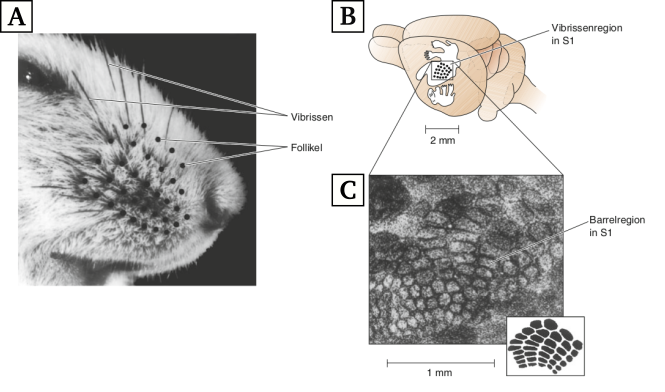
\includegraphics[width = \textwidth] {pictures/somatosensory/barrelcortex.png}
    \caption[Barrelcortex]{\textbf{Barrelcortex.} \textbf{A:} Die Lage der Vibrissen am Beispiel einer Maus. \textbf{B:} schematische Darstellung des primären somatosensorischen Cortex (S1) mit der Lage der 'Barrel' (engl. für Tonne, nach dem Aussehen der einzelnen cortikalen Areale jeder Vibrisse) in S1. Die 'Barrel' sind analog zur Lage der Vibrissen zueinander angeordnet. \textbf{C:} Barrelregion innerhalb von S1. Der Schnitt durch die 'Barrel' ist horizontal zum Cortex angelegt und mit Hilfe einer Nissl-Färbung angefärbt. Die Abbildung unten rechts zeigt erneut die Anordnung der Barrel in fünf Reihen, wie auch in \textbf{A} zusehen ist. \\
    Abbildung aus Aronoff und Petersen, 2008 \textsuperscript{\cite{barrelcortex2008}}.}
    \label{fig:barrelcortex}
\end{figure}

